\documentclass[letterpaper,openright,12pt]{report}
\usepackage[spanish]{babel} % espanol
\usepackage[utf8]{inputenc} % acentos sin codigo
\usepackage{graphicx} % graficos
\usepackage{picture}
\usepackage{booktabs}

\begin{document}

\begin{titlepage}
\setlength{\unitlength}{1 cm} %Especificar unidad de trabajo
\begin{center}
\vspace*{-1in}
\begin{picture}(18,4)
%\begin{center}
\vspace*{0.18in}
\put(0,0){
\includegraphics[width=3cm,height=4cm]{./.imagen/Logoutem.jpg}}
\put(11.5,0){
\includegraphics[width=4cm,height=4cm]{./.imagen/iccilogocolor.png}}
%
\includegraphics[width=4cm]{./.imagen/Logoutem.jpg}
%\end{center}
\end{picture}
\\[2cm]
\textbf{{\Huge Universidad Tecnológica Metropolitana}\\[1.5cm]
{\LARGE Escuela De informática}}\\[1.25cm]
{\LARGE \textbf{Busqueda Mediante Hashing}}\\[2.5cm]
{\large Integrantes:}\\
David Martínez Rivas\\
Felipe Canales Saavedra\\
Javier Reyes Gonzalez\\
Fernando Rubilar Zepeda\\
Profesor:\\
Alejandro Reyes\\[2cm]
Chile - \today
\end{center}

\end{titlepage}
\tableofcontents
\appendix

\newpage
\section{Introducción}

Una \emph{tabla Hash} es una estructura de datos que permite almacenar objetos de distinta índole, los cuales son asociados mediante una clave. La operación principal que es soportada de una manera eficiente, es la búsqueda; que permite el acceso a los objetos (los que pueden ser telefonos, nombres de usuarios, direcciones, etc.) almacenados a partir de una clave generada, a partir del objeto en análisis. Este proceso de transformado se realiza a partir de lo que se conoce como \emph{función hash} que convierte la clave en un hash, es decir, un número que identifica la posición en donde localizar el objeto deseado.

Un ejemplo sencillo para ilustrar lo que es una tabla hash es el siguiente: Se necesita organizar los periódicos que llegan diariamente de tal forma que se puedan ubicar de forma rápida, entonces se hace de la siguiente forma - se hace una gran caja para guardar todos los periódicos (una tabla), y se divide en 31 contenedores (ahora es una "hash table" o tabla fragmentada), y la clave para guardar los periódicos es el día de publicación (índice). Cuando se requiere buscar un periódico se busca por el día que fue publicado y así se sabe en que zócalo (bucket) está. Varios periódicos quedarán guardados en el mismo zócalo (es decir colisionan al ser almacenados), lo que implica buscar en la sub-lista que se guarda en cada zócalo. De esta forma se reduce el tamaño de las búsquedas de $O(n)$ a, en el mejor de los casos, $O(1)$ y, en el peor, a $O(log(n))$.

Básicamente, construir una tabla hash se refiere a una función o método para generar claves o llaves que representan de manera casi unívoca a un documento, registro, archivo, etc., es decir, resumir o identificar un dato a tráves de la probabilidad, utilizando una función hash o algoritmo hash. Siendo entonces un hash el resultado que otorga dicha función o algoritmo%.

\newpage
\section{Historia}

\textbf{Orígenes del término} El término hash proviene, aparentemente,
de la analogía con el significado estándar (en inglés) de dicha palabra
en el mundo real: picar y mezclar. Donald Knuth cree que H. P. Luhn,
empleado de IBM, fue el primero en utilizar el concepto en un memorándum
fechado en enero de 1953. Su utilización masiva no fue hasta después de
10 años. En el algoritmo SHA-1, por ejemplo, el conjunto de partida de
la función es dividido en palabras que son mezcladas entre sí utilizando
funciones matemáticas seleccionadas especialmente. Se hace que el rango
de valores que puede devolver la función sea de longitud fija: 160 bits
utilizando la adición modular.
\newpage



\section{Función hash}

Es una función para resumir o identificar probabilísticamente un gran
conjunto de información, dando como resultado un conjunto imagen finito
generalmente menor. Varían en los conjuntos de partida y de llegada y en
cómo afectan a la salida similitudes o patrones de la entrada.\\\
{Para encontrar la \emph{función hash} no existe una regla que permita
determinar cuál será la función más apropiada para generar un conjunto
de claves que aseguren la máxima uniformidad en la distribución de las
mismas. Algunas de las funciones hash más utilizadas son las
siguientes:}
\begin{itemize}
\itemsep1pt\parskip0pt\parsep0pt
\item
  Función cuadrada.
\item
  Función plegamiento.
\item
  Función truncamiento.
\end{itemize}

La función módulo o por división toma el residuo de la división entre la
clave y el total de elementos de la estructura, generando la siguiente
fórmula: \\[0.4cm]dirección = (clave \% total elementos)\\[0.4cm] Para lograr una mayor
uniformidad en la distribución de los elementos, se debe buscar que el
valor que se usa en el total de elementos sea un número primo más
cercano al tamaño de la estructura. \\Ejemplo. Si tenemos un total de 100
elementos y dos claves que sean 7259 y 9359, las direcciones generadas
son las siguientes: \\[0.4cm]dirección = (7259\%100) = 59 \\dirección = (9359\%100)
= 59 \\[0.4cm]Estos dos casos generan una colisión, ya que los dos números no se
pueden asignar dentro de la misma dirección en la estructura, para
evitar la colisión, se cambia el valor de 100 por el numero primo más
cercano a él, en este caso seria un 97, lo que generaría las siguientes
direcciones:\\[0.4cm] dirección = (7259\%97) = 81 \\dirección = (9359\%97) = 47\\[2.0cm]
La función cuadrada como su nombre lo indica eleva al cuadrado la clave
y del resultado, se toman los dígitos centrales como la dirección. El
número de dígitos a tomar se determina del por el rango del índice de
toda la estructura. La fórmula hash es la siguiente: dirección = dígitos
centrales (clave2) Ejemplo. Si tenemos un total de 100 elementos y dos
claves que sean 7259 y 9359, las direcciones generadas son las
siguientes:\\[0.4cm] dirección = dígitos centrales (72592) = 52693081 = 93\\
dirección = dígitos centrales (93592) = 87590881 = 90\\ 
Como el rango de
claves es de 1 a 100 se toman dos dígitos centrales.\\[0.4cm]
La función plegamiento divide la clave en partes de igual número de
dígitos (la última puede tener menos dígitos), tomando como dirección
los dígitos menos significativos, después de realizar una operación
entre las partes, ya sea una serie de sumas o de multiplicaciones. La
fórmula seria la siguiente:\\[0.4cm] dirección = dígitos menos significativos
(suma de partes)\\ dirección = dígitos menos significativos
(multiplicación de partes)\\[0.4cm] Ejemplo. Si tenemos un total de 100
elementos y dos claves que sean 7259 y 9359, las direcciones generadas
son las siguientes:\\ dirección = dígitos menos significativos (72 + 59)
= dígitos menos significativos (131) = 31\\ dirección = dígitos menos
significativos (93 + 59) = dígitos menos significativos (152) = 52\\[0.4cm]
Como el rango de claves es de 1 a 100 se toman dos dígitos para las
particiones y para la dirección.\\ La función truncamiento toma algunos
de los dígitos de las claves y forma con ellos una dirección. La
elección de los dígitos es arbitraria, podrían tomarse los de las
posiciones pares o impares para con ellos generar la dirección donde se
almacenara la clave, uniendo los dígitos de izquierda a derecha o de
derecha a izquierda, su fórmula es la siguiente:\\[0.4cm] dirección = elegir
dígitos (unión dígitos)\\ Ejemplo. Si tenemos un total de 100 elementos
y dos claves que sean 7259 y 9359, las direcciones generadas son las
siguientes:\\ dirección = elegir dígitos (7, 5) = 75\\ dirección =
elegir dígitos (9, 5) = 95\\[0.4cm] Para este caso se tomaron los dígitos
impares y se unieron de izquierda a derecha.
\newpage

\section{Tratamiento de colisiones}
Las colisiones se dan cuando dos llaves apuntan al mismo índice, resultando en que los registros no pueden ser almacenados en la misma posición. Cuando esto ocurre, se debe buscar otra localización para almacenar el nuevo registro, y hacerlo de tal manera que sea posible encontrarlo.

Para dar una idea de la importancia de utilizar una buena estrategia para hacer frente a las colisiones, es bueno considerar que si tenemos un millón de registros, es factible en un 95\% tener al menos una colisión antes de alcanzar las 2500 entradas.

En la literatura, es posible encontrar diferentes técnicas para resolver este problema, sin embargo las resoluciones más populares son las siguientes:
\begin{itemize}
\itemsep1pt\parskip0pt\parsep0pt
\item
  Direccionamiento cerrado o Hashing abierto: En la técnica más simple de encadenamiento, cada casilla en el array referencia una lista de los registros insertados que colisionan en la misma casilla. La inserción consiste en encontrar la casilla correcta y agregar al final de la lista correspondiente. El borrado consiste en buscar y quitar de la lista.
  Otras estructuras de datos pueden ser utilizadas para el encadenamiento en lugar de las listas ligadas. Al usar árboles auto-balanceables, por ejemplo, el tiempo teórico del peor de los casos disminuye de O(n) a O(log n). Sin embargo, dado que se supone que cada lista debe ser pequeña, esta estrategia es normalmente ineficiente a menos que la tabla hash sea diseñada para correr a máxima capacidad o existan índices de colisión particularmente grandes. También se pueden utilizar vectores dinámicos para disminuir el espacio extra requerido y mejorar el rendimiento del caché cuando los registros son pequeños.
\newpage
\item
  Direccionamiento abierto o Hashing cerrado: Las tablas hash de direccionamiento abierto pueden almacenar los registros directamente en el array. Las colisiones se resuelven mediante un sondeo del array, en el que se buscan diferentes localidades del array (secuencia de sondeo) hasta que el registro es encontrado o se llega a una casilla vacía, indicando que no existe esa llave en la tabla.
\end{itemize}
  Las secuencias de sondeo más utilizadas son:
\begin{itemize}
\itemsep1pt\parskip0pt\parsep0pt
\item
Sondeo lineal.
\item
Sondeo cuadrático.
\item
Doble Hasheo.
\end{itemize}

El sondeo lineal ofrece el mejor rendimiento del caché, pero es más sensible al aglomeramiento, en tanto que el doble hasheo tiene pobre rendimiento en el caché pero elimina el problema de aglomeramiento. El sondeo cuadrático se sitúa en medio. El doble hasheo también puede requerir más cálculos que las otras formas de sondeo.

\newpage

\section{Análisis de complejidad}

Como se dijo anterior mente el hashing de direccionamiento cerrado, es la política más sencilla para manejar colisiones,motivo por el cual será objeto de estudio en este informe.
Entonces, para poder insertar un elemento en el hash, se calcula su valor de dispersión (clave), digamos $i$, y se inserta en la tabla $H(i)$ (que puede ser una lista ligada, un árbol, un vector, etc.). Si la tabla contiene $n$ elementos y $h$ es el tamaño de la tabla, entonces podremos decir que su \emph{factor de carga} se define como: \begin{equation}
\alpha = n/h
\end{equation} Siendo $\alpha$ la razón entre cantidad de datos y tamaño de la tabla.
Para este caso, no es posible suponer que dada una clave, obtendremos el valor que se requiera, ya que varios de estos pueden tener asociada una misma clave. Convirtiendo la función en una del tipo \emph{"muchos a uno"}.

Supóngase que es igualmente probable que tengamos que buscar cualquier elemento de latabla, y que en ella se han almacenado $n$ elementos. ¿Qué costo medio tiene una búsqueda exitosa? Supóngase que el costo de calcular el código de dispersión es igual al costo de efectuar un número pequeño, digamos $a$, de comparaciones de claves. Si el hashing coloca a un elemento en la celda $i$, cuya lista ligada tiene $L_i$ elementos, entonces el número medio de comparaciones necesarias para hallar el elemento será $(L_i + 1)/2$. En tal caso, el costo medio de una búsqueda exitosaestará dado por:
\begin{equation}
a + 1/h \sum_{i=0}^{h-1}(L_i + 1)/2
\end{equation}
\newpage
\begin{center}
\begin{figure}[h]
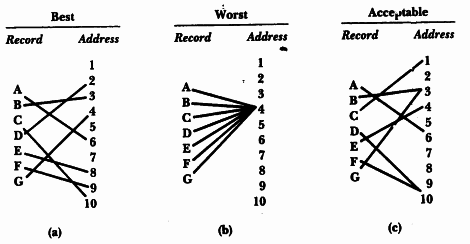
\includegraphics[width=265px,height=152px]{./.imagen/colision_case.png}
\end{figure}
\end{center}
Supongamos que se tiene un factor de dispersión de $n/10$, una búsqueda exitosa requerirá entonces de $n/200$ comparaciones de claves. En el peor de los casos, \emph{todos} los elementos se acomodarán a una misma celda y, por lo tanto, una búsqueda exitosa requerirá en promedio $n/2$, o $O(n)$, es decir, demorará lo mismo que si se estuviera realizando la búsqueda en un arreglo de elementos no ordenados. Estos casos se dan cuando la función hash no está bien implementada.
El mejor de los casos, es cuando las claves que se obtienen de los objetos tienen la probabilidad de pertenecer al intervalor $0, ..., h - 1$. Aquí una búsqueda exitosa requiere en promedio $O(1 + \alpha)$. Y si dentro del factor de carga nuestro $h$ es proporcional a $n$ entonces, en promedio se necesitarán $O(1)$ comparaciones de claves para lograr una búsqueda.



\newpage


\section{Propiedades de la función hash}

La calidad de la función hash, está definida en base a ciertas propiedades (no necesariamente todas deben cumplirse) según el contexto en el cual se esté trabajando, las cuales son:
\begin{itemize}
\itemsep1pt\parskip0pt\parsep0pt
\item
  Bajo costo: Calcular el valor hash de un objeto, necesita poco costo computacional (memoria).
\item
  Compresión: Una función hash comprime datos si puede mapear un dominio con datos de longitud muy grande a datos con longitud más pequeña.
\item
  Uniformidad: Se dice que una función hash es uniforme cuando para una clave elegida aleatoriamente es igualmente probable tener un valor hash determinado, independientemente de cualquier otro elemento.
\newpage
\item
  Rango variable: En algunos casos, el rango de valores hash que maneje la función pueden ser diferentes a lo largo del tiempo. Este caso se da cuando, en función del tiempo, la tabla hash necesita expandir su capacidad de almacenamiento. Para estos casos, a la función hash se le indica un parámetro que alerte de estos escenarios.
\item
  Inyectividad (Perfección): La función hash que es perfecta, se dice que es inyectiva (esto ocurre cuando a cada dato le corresponde una clave diferente con respecto a otro). Para que pueda existir esta condición, es necesario que la cardinalidad del conjunto de objetos sea inferior a la del conjunto imágen. En la realidad es muy poco probable que ocurra esto, normalmente se da cuando se ingresan entradas preestablecidas. Por ejemplo: Ingresar los números del 1 al 100 por orden de aparición.
\item
  Determinismo: Una función hash se dice que es determinista cuando dada una cadena de entrada siempre devuelve el mismo valor hash. Es decir, el valor hash es el resultado de aplicar un algoritmo que opera sólo sobre la cadena de entrada. Ejemplos de funciones hash no-deterministas son aquellas funciones hash que dependen de parámetros externos, tales como generadores de números pseudoaleatorios o la fecha. Tampoco son deterministas aquellas funciones hash que dependen de la dirección de memoria en la que está almacenada la cadena de entrada. Esa dirección es accidental y no se considera un cambio de la cadena entrada en sí. De hecho puede cambiar dinámicamente durante la propia ejecución del algoritmo de la función hash.
\end{itemize}
\newpage

\section{Ventajas y desventajas de la función hash}
\subsection{Ventajas}

Se pueden usar los valores naturales de la llave, puesto que se traducen
internamente a direcciones fáciles de localizar Se logra independencia
lógica y física, debido a que los valores de las llaves son
independientes del espacio de direcciones No se requiere almacenamiento
adicional para los índices.

\subsection{Desventajas}

El archivo no esta clasificado No permite llaves repetidas Solo permite
acceso por una sola llave Costos Tiempo de procesamiento requerido para
la aplicación de la función hash
\newpage

\subsection{Mediciones de tiempo}
A continuación se presentan las mediciones de tiempo de los algoritmos: Mejor caso, peor caso y caso promedio.

\subsubsection{Mejor caso}
\begin{center}
\begin{table}[h]
\begin{tabular}{lll}
Cantidad de datos & Dato a buscar & Tiempo de ejecución(ms)\\
1000   & 993 & 0.00500679 \\
10000  & 993 & 0.00715256 \\
100000 & 993 & 0.00691414
\end{tabular}
\end{table}
\end{center}
Para el mejor caso, no es de importancia verificar con mayor cantidad de datos, dado que la complejidad de búsqueda siempre será constante, $O(1)$, es decir, siempre, la búsqueda, va directo al dato que se requiere. Este es el clásico ejemplo de la función hash perfecta (a cada dato le corresponde una única clave).

\subsubsection{Caso promedio}
\begin{center}
\begin{table}[h]
\begin{tabular}{lll}
Cantidad de datos & Dato a buscar & Tiempo de ejecución(ms)\\
1000 & 333     & 0.00596046 \\
10000 & 4596    & 0.0200272  \\
100000 & 45946   & 0.00619888 \\
1000000 & 345234  & 0.0119209  \\
10000000 & 4543456 & 0.00882149
\end{tabular}
\end{table}
\end{center}
En este caso, se ve una demora en el acceso de los datos, dado que se encuentran mayores colisiones para cada clave generada por los datos. Lo que va transformando cada búsqueda en una del tipo $O(n)$ o $O(log(n))$
\newpage

\subsubsection{Peor Caso}
\begin{center}
\begin{table}[h]
\begin{tabular}{lll}
Cantidad de datos & Dato a buscar & Tiempo de ejecución(ms)\\
1000 & 207      & 0.00786781 \\
10000 & 8314    & 0.0190735  \\
100000 & 70823    & 0.0691414 \\
1000000 & 805591  & 0.0905991 \\
10000000 & 9999736  & 0.169277 
\end{tabular}
\end{table}
\end{center}
La búsqueda de un elemento en el peor de los casos, toma aproximadamente $n/2$ o $O(n)$ comparaciones de claves, un pésimo resultado. Ya que estos no son mejores como los que se dan en un arreglo no ordenado. Mostrando lo importante que es el hecho de escoger una muy buena función hash.




\newpage

\section{Aplicación}

\begin{itemize}
\itemsep1pt\parskip0pt\parsep0pt
\item
  Es posible que existan claves resultantes iguales para objetos
  diferentes, ya que el rango de posibles claves es mucho menor que el
  de posibles objetos a resumir (las claves suelen tener en torno al
  centenar de bits, pero los ficheros no tienen un tamaño límite).
\item
  Son usadas en múltiples aplicaciones, como los arrays asociativos,
  criptografía, procesamiento de datos y firmas digitales, entre otros.
  Una buena función de hash es una que experimenta pocas colisiones en
  el conjunto esperado de entrada; es decir que se podrán identificar
  unívocamente las entradas.
\item
  Las tablas hash, una de las aplicaciones más extendidas de las
  funciones de hash, aceleran el proceso de búsqueda de un registro de
  información según una clave (nota: este uso de la palabra poco se
  relaciona con su significado habitual). Por ejemplo, una cadena
  alfanumérica puede ser utilizada para buscar la información de un
  empleado en la base de datos de un sistema.
\item
  La utilización de tablas hash provee un acceso casi directo a dichos
  registros, lo que significa que, en promedio, una búsqueda puede
  llegar a requerir sólo uno o dos intentos en la memoria o el archivo
  que contiene la información. Naturalmente, se prefiere una buena
  función de hash que evitará colisiones de hash.
\item
  Si asumimos que la clave es una cadena de bytes, entonces la función
  de hash debería ser como un índice de los registros que tiene una
  distribución aleatoria sobre las cadenas de entrada esperadas. De otra
  forma, habría más colisiones de hash degradando así el tiempo de
  búsqueda. Si, por ejemplo, la clave es alfabética, cada byte puede
  tener sólo 26 de sus 256 valores posibles. Funciones tan simples no
  distribuirán los índices de una forma pareja.
\item
  Para una comparación de velocidad y calidad de varias funciones de
  hash, referirse a los enlaces externos.
\end{itemize}
\newpage
\section{Conclusión}

Las funciones criptográficas hash juegan un papel fundamental en la criptografía moderna. Hay muchas funciones hash, comúnmente usadas en aplicaciones no criptográficas. Nosotros nos referiremos siempre a las que admiten el adjetivo de criptográficas, y las llamaremos habitualmente simplemente funciones hash. 

A continuación se presentan una serie conclusiones:

\begin{itemize}
\itemsep1pt\parskip0pt\parsep0pt

\item
Comparada con otras estructuras de arrays asociadas, las tablas hash son más útiles cuando se almacenan grandes cantidades de información.

\item
El método de búsqueda hash o por transformación de clave aumenta la
velocidad de búsqueda sin necesidad de que los elementos estén
previamente ordenados.

\item
Pueden ser utilizadas en el área de la criptografía, en este caso, son llamadas \emph{funciones hash criptográficas}.

\item
Si bien, este mpetodo es útil para un gran volúmen de datos, es necesario implementar una buena función de dispersión. De esta manera se aseguran que los datos queden repartidos por toda la tabla de manera uniforme y también se reducen las colisiones posibles.

\item
Como ya sabemos, este método es ultilizado para almacenar datos. Pero gracias la función hash, este mismo puede ser utilizado en varios campos:
\begin{itemize}
\itemsep1pt\parskip0pt\parsep0pt
\item
Como herramienta base para construir estructuras más complejas.
\item
Forma de proteger la integridad de los datos a transmitir (checksum).
\item
Herramientas vinculadas a la autenticación y cntrol de acceso.
\item
Formas para la identificación y la rápida comparación de datos.
\end{itemize}
\end{itemize}
\end{document}
